\documentclass[pdftex,twoside,a4paper]{report}
\usepackage[pdftex]{graphicx}
\usepackage[margin=3.0cm]{geometry}
\usepackage{times}
\usepackage[english]{babel}
\usepackage[normalem]{ulem}
\usepackage{algorithm2e}
\usepackage{amsfonts}
\usepackage{amsmath}
\usepackage{amssymb}
\usepackage{tabularx}
\usepackage{color}
\usepackage{tabto}
\usepackage{graphicx}
\usepackage{hyperref}
\usepackage{float}
\usepackage{epstopdf}
\usepackage{caption}
\usepackage{subfigure}
\newcommand{\hilight}[1]{\colorbox{yellow}{#1}}
\newcommand{\TODO}{\hilight{NOT DONE}}
\newcommand{\hs}{$\hspace{0.5cm}$}
\newcommand{\bt}{\begin{tabbing}}
\newcommand{\et}{\end{tabbing}}
\newcommand{\bcen}{\begin{center}}
\newcommand{\ecen}{\end{center}}
\newcommand{\length}{\ell}
\newcommand{\pmem}{Particle Mesh Ewald method}
\newcommand{\fma}{Fast Multipole Algorithm}

\begin{document}

\begin{titlepage}
 
\begin{center}


\includegraphics[width=0.8\textwidth]{logoWhite.png}\\[0.5cm]
\textsc{\Large Research School of Computer Science}\\[0.5cm]
\textsc{\Large College of Engineering and}\\[0.2cm]
\textsc{\Large Computer Science}\\[0.5cm]


 
\vspace{1.4cm}

\hrule

\vspace{1.4cm}

{ \huge \bfseries The Fast Multipole Algorithm vs. the Particle Mesh Ewald method} \\

\vspace{0.4cm}

{ \LARGE \bfseries Joshua Nelson - u4850020} \\

\vspace{1.4cm}


\hrule

\vspace{1.0cm}

\textsc{\large COMP3006 - Computer Science Research Project}\\

\vspace{1.0cm}

\hrule

\vspace{1.4cm}



\emph{Supervisor: } 
Dr Eric \textsc{McCreath} \\

 
\vfill
 
% Bottom of the page
{\large \today}
 
\end{center}
 
\end{titlepage}



\begin{abstract}
The N body problem is common across the fields of physics, biology and chemistry. The classic solution to this problem has an inhibitive complexity in the class $O(n^2)$. Two alternative methods were examined: The Fast Multipole Algorithm, and the Particle Mesh Ewald Method, with better complexities of $O(n)$ and $O(n \text{log}(n))$, respectively. These algorithms were implemented in Java, and their efficiencies were discussed and compared. The algorithms were run over typical molecular dynamics simulations to determine the most efficient algorithm for the N-body problem.
\end{abstract}

\tableofcontents

%_____________INTRODUCTION CHAPTER________________
\chapter{Introduction}
This chapter introduces the N body problem, approaches that have been made in the past, and gives background on related literature.
\section{The N body problem}
    \subsection{Problem summary}
    Suppose we have a collection of $n$ bodies in some space, that interact with each other. Each body interacts with every other body in the system in a pairwise way. Often this pairwise interaction is a function of the distance between the bodies, and their properties, such as mass or electric charge. The task is to calculate the total effect on each body from every other body.\\
    
    The N body problem is key to the simulation of many different scientific environments. The bodies may be astrophysical objects, such as planets or galaxies, interacting based on distance and body mass \cite{MilleniumRun}, or atoms in a molecular dynamics simulation, based on distance and particle charge.\cite{NAMD}. During the report, we will mostly discuss the N body problem in regards to Molecular dynamics, however the approaches can be generalised to other fiields.
    \subsection{History of the problem}
    The N body problem was first formulated mathematically in Isaac Newton's Principia Mathematica. \cite{principia}. Later, H. Poincar\`{e} showed the impossibility of an analytical solution using first order integrals for $N \geq 3$. \cite{poincare}. This led to the development of several approximation methods. These methods can be roughly classified as either tree methods, or mesh methods.\\
    
    Tree methods are methods that break the simulation space into cells, and use a tree structure to organise these cells, allowing close interactions to be calculated directly, and far ones approximated. The \fma{}, first described by L. Greengard and V. Rokhlin \cite{greengard:315}, is such a method, using multipole expansions to approximate far cells.\\
    
    Mesh methods are ones that discretize the simulation space onto a mesh, and the potential is then solved over the mesh. The \pmem{}, developed by T. Darden et al.\ \cite{darden:10089} is such a method, and is based on Ewald summation, developed by P. Ewald \cite{ewald}. The variation of this known as the Smooth \pmem{} was developed by U. Essman et al.\ \cite{essmann:8577}\\
    \subsection{Related work}
    Comparisons of the \fma{} and the \pmem{} that have been made previously have found that the \pmem{} outperforms the \fma{} in the range $10^4$ - $10^5$. (H. Petersen, \cite{petersen:3668}). A. Toukmaji et al.\ \cite{toukmaji:73} claim that the mesh methods are faster in the range $10^3$ - $10^4$, and the multipole tree methods faster for $N > 10^5$.
    \subsection{Contribution}
    The contribution to this section of work that this paper provides includes a basic Java implementation of the \pmem{} and the \fma{}. This software allows direct comparison of the two algorithms in terms of speed and accuracy. The code was written with readibility in mind, rather than focusing on excessive optimisation, which obscures the algorithm the code implements.
    
    The report seeks to give insight into the approaches from a Computer Science perspective, while giving the background necessary to understand it from a Computational Chemistry perspective.
    
    
    

%_____________ALGORITHMS CHAPTER________________
\chapter{Algorithms for the N body problem}
This chapter describes the mathematics and the implementation of the main algorithms discussed in this report: The basic algorithm, the \fma{}. and the \pmem{}. For each of these methods, we examine their running times and accuracy individually, and discuss the details of their implementations in Java.
\section{The $O(n^2)$ solution}
\subsection{The algorithm}
        
%%%%%%%%FIGURE%%%%%%%%%%%%%
\begin{figure}
\bcen 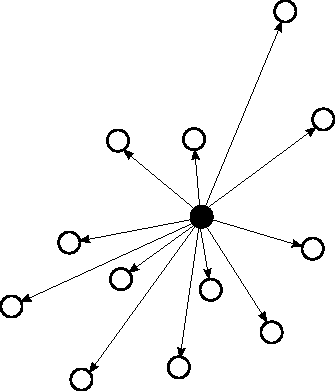
\includegraphics{figures/nbodies.pdf} \ecen
\caption{The na\"{\i}ve approach to the n body problem - calculate each interaction for each particle}
\label{fig:basic_alg_diag}
\end{figure}

The simplest solution to the N body problem is the basic $O(n^2)$ approach of calculating each interaction directly (See Figure \ref{fig:basic_alg_diag}). Pseudocode for this soltuion is given in Algorithm \ref{alg:basic}.\\

%%%%%PSEUDOCODE%%%%%%%%%
\begin{algorithm}
 \SetLine
 \KwData{$r_i$: particle positions, $q_i$: particle charges, N: number of particles, Q: output array of charges}
 \For{i=0 to N}{
  \For{j=i to N}{
      \If{$i \not= j$}{
        $d := |r_i - r_j|$\;
        $Q[i] := q_i * q_j / d$\;
       }
  }
 }
 \caption{The basic approach to the N body problem}
 \label{alg:basic}
\end{algorithm}

The advantages to the $O(n^2)$ approach are it's simplicity, ease of implementation, and it's low initialisation overhead. This low overhead can be seen in Figure \ref{fig:basic_algo_complex}. However, it's primary disadvantage is that it is limited to small numbers of particles by it's $O(n^2)$ complexity. These advantages and disadvantages are further discussed in Chapter \ref{chap:compare}

\subsection{Implementation analysis}
The $O(n^2)$ algorithm was run on increasing system sizes for one time step, and the time taken to calculate the potential at each atom's position was calculated. It is easy to turn this process into a dynamic simulation, using the relationship between potential energy, a particle's charge, and force.
%%%%%%%%FIGURE%%%%%%%%%%%%%
\begin{figure}
\bcen 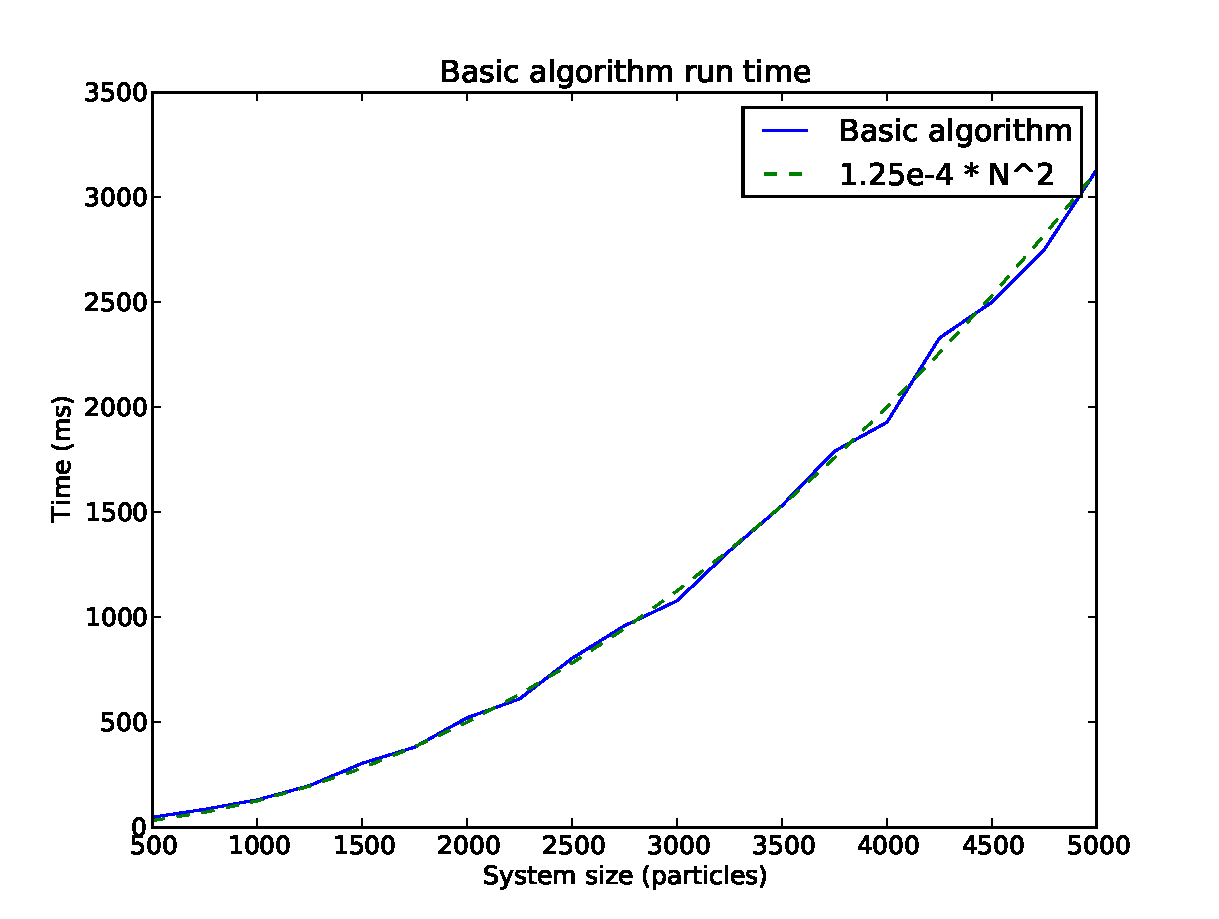
\includegraphics[width=0.75\textwidth]{figures/graphs/basic_algo_complex.pdf} \ecen
\caption{The basic algorithm's run time compared to a function of $N^2$. It is easy to see that the basic algorithms run time grows proportionally to $N^2$, as we would expect from it's complexity class $O(n^2)$}
\label{fig:basic_algo_complex}
\end{figure}

We can see in Figure \ref{fig:basic_algo_complex} that the running time increases porportionally to $N^2$. We can also see the low overhead when N is in the range $N < 1000$, where the total computation time $\approx 100$ms.

Details of the computer these measurements were taken on can be found in Appendix \ref{ap:implement}. By sampling Figure \ref{fig:basic_algo_complex} at various points, we find that the rate of computation for the implementation is approximately 38.9 Mflops.

%_____________PME Section________________
\section{The particle mesh ewald method}
\subsection{Background}
\subsubsection{Potential vs. Energy}
Energy and potential are related but different concepts. They both describe effects charged particles have on their surrounding environment, however, \emph{Energy} is a property of a particle, and \emph{Potential} is a property of a field. \emph{Energy} is defined in terms of a particle-particle interaction, while \emph{Potential} describes a field from one charged particle.\\
Coulomb's law describes the potential at $r_2$ from a charge $q_1$ at $r_1$ as 
\[V=\frac{1}{4\pi \epsilon_0} \frac{q_1}{|r_2 - r_1|}\]
And energy from a particle with charge $q_2$ at $r_2$ as $E = q_2 V$.\\
For our purposes, the constant term $\frac{1}{4\pi \epsilon_0}$ is material dependent, and is discarded.
\subsubsection{Ewald summation}
The key concept behind the \pmem{} is that of \emph{Ewald Summation}. Ewald Summation splits the potential $\phi$ at a position $r$ into two components, the long range potential and the short range potential. \cite{petersen:3668}.
\[
\phi(r) = \phi_{\text{sr}}(r) + \phi_{\text{lr}}(r)
\]
The advantage of doing this is that $\phi_{\text{sr}}$, the short range term, converges quickly in real space (effects from charges far away from $r$ quickly decrease), while $\phi_{\text{lr}}$ converges quickly in reciprocal space. The \pmem{} takes advantage of this by calculating the $\phi_{\text{sr}}$ term by calculating potential directly for nearby particles, and uses a grid based direct fourier transformation to calculate the long range component.
\subsubsection{Real space computation}
The short range potential at a point can be computed by considering only particles within a small radius of the point. We can keep the radius small as $\phi_{\text{sr}}$ converges quickly in real space. This is also important, as we need to keep the number of particles considered less than $N$, in order to reduce the algorithm from $O(n^2)$ to $O(n)$ complexity. This is the case though, as the radius we consider is constant and less than the size of the simulation cell width, and we assume the particles are distributed randomly within the simulation cell.
%%%%%%%%FIGURE%%%%%%%%%%%%%
\begin{figure}
\bcen 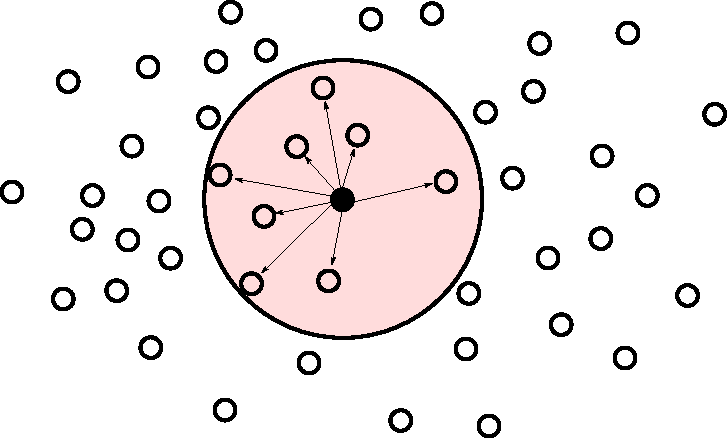
\includegraphics{figures/cutoff.pdf} \ecen
\caption{A particle and the particles that we consider it's interactions with, based on the cutoff distance}
\end{figure}

\subsubsection{Reciprocal space computation}
The reciprocal space is the long range part of the potential computation, which converges slowly in real space. However, in reciprocal space, it converges quickly, so we use discrete fourier transformations to calculate this part of the sum.\\

Discrete fourier transformations require a discrete space to transform, however, our real space is continuous. So for this, we need to discretise the charges onto a grid. The approach taken in the original paper was to use Lagrangian interpolation to achieve this. Close mesh cells receive most of the charge from each particle, and this amount decreases to zero at some point, depending on the interpolation order. This is described in detail in Section \ref{sec:math_desc_lagrange}.\\
%%%%%%%%FIGURE%%%%%%%%%%%%%
\begin{figure}
\bcen 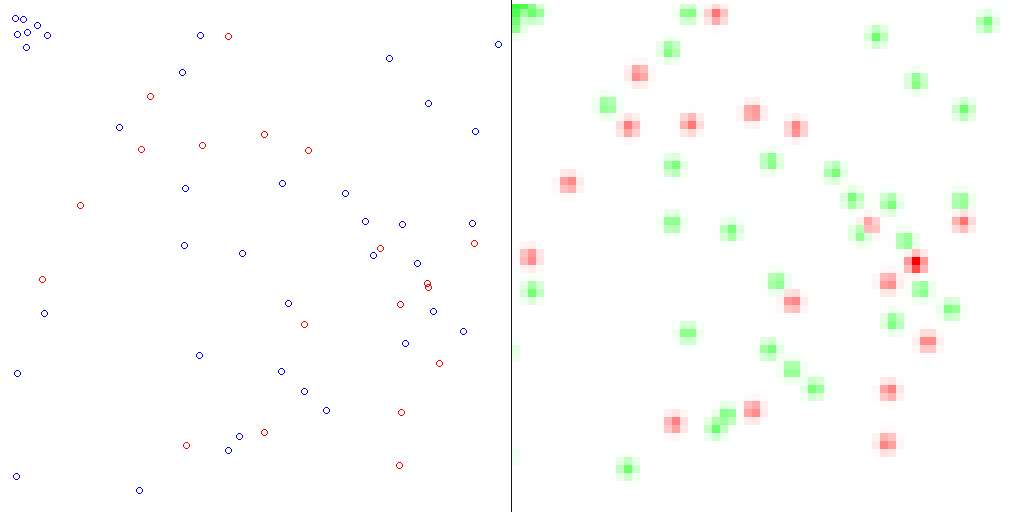
\includegraphics[width=\textwidth]{figures/Qarray.jpg} \ecen
\caption{A distribution of continuous charges, and an interpretation of them as discrete charges}
\end{figure}

An alternative to using lagrange interpolation is to use cardinal B splines. This modification is known as the \emph{Smooth Particle Mesh Ewald} method, and is advantageous in terms of accuracy, and is also easily differentiable, which is important if the forces are required as well as the potentials.  \cite{essmann:8577} This is the method that was implemented in this paper.


\subsubsection{Periodic boundary conditions}
\label{sec:pme_period_bound_cond}
One feature of the \pmem{} is the ability to simulate \emph{Periodic Boundary Conditions} \cite{essmann:8577}. Periodic Boundary Conditions have a wrap around behaviour - that is, instead of treating the walls of the simulation unit as empty space, we can allow them to loop around to the other side of the box again, effectively allowing infinite replication of the simulation unit (See Figure \ref{fig:pme_pbc}) This is helpful practically, as many applications are interested in the effects on a small portion of a large system \cite{toukmaji:73} (For example, simulation of water at a molecular scale). Simulating the entire system would be time consuming if not impossible, and simulating only a small portion without Periodic Boundary Conditions would produce unrealistic results (Molecules may disperse into empty space over time). While useful practically, Periodic Boundary Conditions do not change the complexity or performance, and as our interest is in a comparison with the \fma{}, we reduce the effects of Periodic Boundary Conditions by placing all particles within a larger, mostly empty, simulation cell. This extra padding mostly negates the effects of the Periodic Boundary Conditions.
%%%%%%%%FIGURE%%%%%%%%%%%%%
\begin{figure}
\bcen 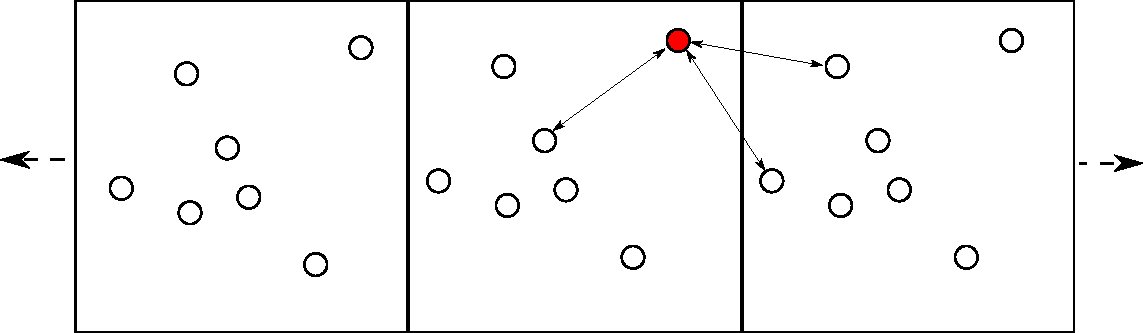
\includegraphics[width=0.75\textwidth]{figures/pbc.pdf} \ecen
\caption{A particle interacting with it's nearest neighbours, with periodic boundary conditions in one dimension (x axis)}
\label{fig:pme_pbc}
\end{figure}

\subsection{Mathematical description}
\subsubsection{Interpolating the charges to the Q array}
\label{sec:math_desc_lagrange}
We first present the formulation of the Q array based on lagrangian interpolation. 
\begin{equation} \label{eq:q_array}
Q(k_x,k_y) = \sum_{i=1} ^N q_i W_{2p}(u_{xi} - k_x) * W_{2p}(u_{yi} - k_y)
\end{equation}
Where,
\begin{itemize}
    \item $N$ is the number of particles,
    \item $n_1,n_2$ are integers $< N$,
    \item $W_{2p}$ is a Lagrangian polynomial of order $p$ with a value in the range $[0,1]$,
    \item $K$ is the number of cells we split the grid into,
    \item $u_{xi}, u_{yi}$ are scaled fractional coordinates of particle $i$ (Scaled fractional coordinate coordinates meaning $u_{xi} = K * (r_{xi} / (\text{simulation width}))$, $r_{xi}$ is the particle i's $x$ coordiante, so $0 \leq u_{xi} \leq K$).
\end{itemize}
More information can be found in \cite{essmann:8577}.\\

We can replace $W_{2p}$ in the above with $M_n$, a cardinal B spline of order $n$, and the formulation of the Q array is the same. This modification is known as the Smooth \pmem{}. From this point forward, we will use cardinal B spline interpolation. The mathematics of B spline interpolation is described in Appendix \ref{sec:eval_bspline}


\subsubsection{Calculating electrostatic potential from the Q array}
With this Q array we can calculate the long range contribution to the electrostatic potential in reciprocal space.\\

\begin{equation}
E_{\text{rec}} = \frac{1}{2} \sum_{m_1 = 0}^K \sum_{m_2 = 0}^K Q(m_1,m_2) * (\theta_{\text{rec}} \star Q)(m_1,m_2)
\label{eq:energy_rec}
\end{equation}
With $\theta_{\text{rec}} = F(B * C)$, and so $(\theta_{\text{rec}} \star Q)(m_1,m_2) = F(B * C * F^{-1}(Q))$\\
Where $C$ is the matrix for the original exponential term from Equation \ref{eq:ap_primitive_rec_energy}, that is,
 \bcen
$\displaystyle
C(m_1,m_2) = \frac{1}{\pi V} \frac{\text{exp}(- \pi^2 m^2 / \beta^2)}{m^2} $ for $ m \not= 0, C(0,0) = 0$
\ecen

Details on the derivation of this equation can be found in Appendix \ref{ap:deriv_rec_energy}, \cite{essmann:8577}, \cite{lee05}.

\subsubsection{Interpolating energies back from the mesh in real space}
\label{sec:interpolate_from_grid}
If we have a point $r$ in real space that we wish to calculate the potential for, we can interpolate back from a mesh in the same way we did while creating the discrete mesh.
That is, with $r = (r_x,r_y)$, which has scaled fractional coordinates $(u_x,u_y)$ (see Section \ref{sec:math_desc_lagrange}), at point $r$ we have\\
\begin{equation}
\label{eq:interpoalte_from_grid}
E(r_x,r_y) = \sum _{i,j = -n} ^{n} Q(\lfloor u_{x+i} \rfloor,\lfloor u_{y+j} \rfloor) * M_n(u_x - \lfloor u_{x+i} \rfloor) * M_n(u_y - \lfloor u_{y+j} \rfloor)
\end{equation}
This equation iterates over cells within our interpolation order $n$, and calculates the weighting we ascribe to the cell ($ M_n(u_x - \lfloor u_{x+i} \rfloor) * M_n(u_y - \lfloor u_{y+j} \rfloor$, a real number in the range $[0,1]$). Summing the proportion of the grid charge assignments, we produce B Spline interpolated values from the grid.
\subsubsection{The ewald coefficient}
The ewald coefficient, $\beta$, is a number describing the ratio between the real space and the reciprocal space contributions to the calculation of the total energy. In practice, it depends on the tolerance $\epsilon_\text{tol}$, and our desired cutoff distance $r_{\text{cut}}$ in the following way, \cite{darden:10089} \cite{essmann:8577}\\
\begin{equation}
\frac{\text{erfc}(\beta r_{\text{cut}})}{r_\text{cut}} \leq \epsilon_\text{tol}
\label{eq:ewald_coeff}
\end{equation}
Where erfc is the complimentary error function, a function that tends quickly to zero, depending on it's argument. The relation means that for $r > r_{cut}$, we have $\frac{\text{erfc}(\beta r_{\text{cut}})}{r_\text{cut}} \leq \epsilon_\text{tol}$, and for all $r > r_\text{cut}$ we can ignore the direct energy contribution, given by equation \ref{eq:energy_dir} \cite{essmann:8577}\\
\begin{equation}
E_\text{dir} = \frac{1}{2} \sum_{n} \sum_{i,j = 1} ^N \frac{q_i q_j \text{erfc}{\beta |r_j - r_i|}}{|r_j - r_i|}
\label{eq:energy_dir}
\end{equation}
Which becomes approximately
\begin{equation}
E_\text{dir} \approx \frac{1}{2} \sum_{n} \sum_{i,j = 1} ^{\overset{*}{N}} \frac{q_i q_j}{|r_j - r_i|}
\label{eq:energy_dir_noerfc}
\end{equation}
Where the $*$ indicates terms with $|r_j - r_i| > r_{\text{cut}}$ are left out of the sum





\subsection{The algorithm}
\subsubsection{Main particle mesh ewald flow}
The basic flow of the algorithm is given in Algorithm \ref{alg:pme} \newline
%%%%%PSEUDOCODE%%%%%%%%%
\begin{algorithm}[H]
\label{alg:pme}
\SetLine
\KwData{$Q$: Charge assignment matrix, $r_{\text{cut}}$: Cutoff distance, $r$: position at which we calculate the potential}
Initialise the ewald coefficient (Equation \ref{eq:ewald_coeff}, algorithm in Appendix \ref{sec:alg_ewald_coeff})\\
Calculate the B spline coefficients (Details in \cite{essmann:8577} \cite{lee05})\\
Allocate particles to their cells (Using a Verlet list, see section \ref{sec:verlet})\\
Initialise the Q matrix (Equation \ref{eq:q_array})\\
Calculate reciprocal energy (Equation \ref{eq:energy_rec})\\
Calculate direct energy (Equation \ref{eq:energy_dir})\\
Interpolate reciprocal energies back to desired coordinates (Section \ref{sec:interpolate_from_grid})\\
\For{Every particle $p$ within $r_{\text{cut}}$ of $r$ (Calculate using Verlet list, (Section \ref{sec:verlet})}{
Caclulate and sum the direct potential from $p$ at $r$.
}
Combine the interpolated energy and directly computed energy
\caption{The Particle Mesh Ewald Method}
\end{algorithm}

\subsection{The implementation}
The \pmem{} was implemented in Java, with a GUI front end. In this section, we break down the \pmem{}, and look at the interesting data structures and methods used in initialisation and potential calculations.

\subsubsection{The Cardinal B Spline}
The Cardinal B Spline was implemented by means of recursion. The class \texttt{BSpline.java} contains the methods required for evaluating the B Spline and it's derivative, as well as the Euler Exponential splines (Described in Eq. \ref{eq:ap_primitive_rec_energy}). This recursion is performed many times, and is costly at high accuracies (high B Spline orders). This makes it a target for optimisation (See section \ref{sec:optimisations})
\subsubsection{Fast Fourier Transformations}
The chosen library for Fast Fourier Transformations (Required for calculation of the reciprocal space potential) was the JTransforms library\footnote{JTransforms FFT Library, \url{http://sourceforge.net/projects/jtransforms}}. This library has the advantage of being implemented in pure Java code, allowing simpler integration and debugging. The Fourier Transformation operation is the core of the run time for the \pmem{}, and so and optimised library is essential for performance reasons.
\subsection{Running time analysis}
\subsubsection{Cardinal B spline}
\label{sec:optimisations}
%TODO: recursive defintion given where?
With a basic implementation of the B spline, implemented directly from the recursive definition given, we notice a dramatically decreased run time. Computing the B spline coefficients is costly in terms of time, and must be computed repeatedly. A method to reduce this running time was implemented, with a HashMap saving values that had already been evaluated. This hash table had a hit rate of approximately $98\%$, as we evaluate fractional coordinates for the same particles often in the \pmem. The hash function converted the double keys to integer keys, which provides some collisions, but the B spline function is smooth, so similar $x_1, x_2$ values produce similar $M_n(x_1)$ and $M_n(x_2)$ values. The goal of this was to reduce the running time, as hashing full doubles is expensive.
\subsubsection{Algorithm complexity}
%%%%%%%%FIGURE%%%%%%%%%%%%%
\begin{figure}
\bcen 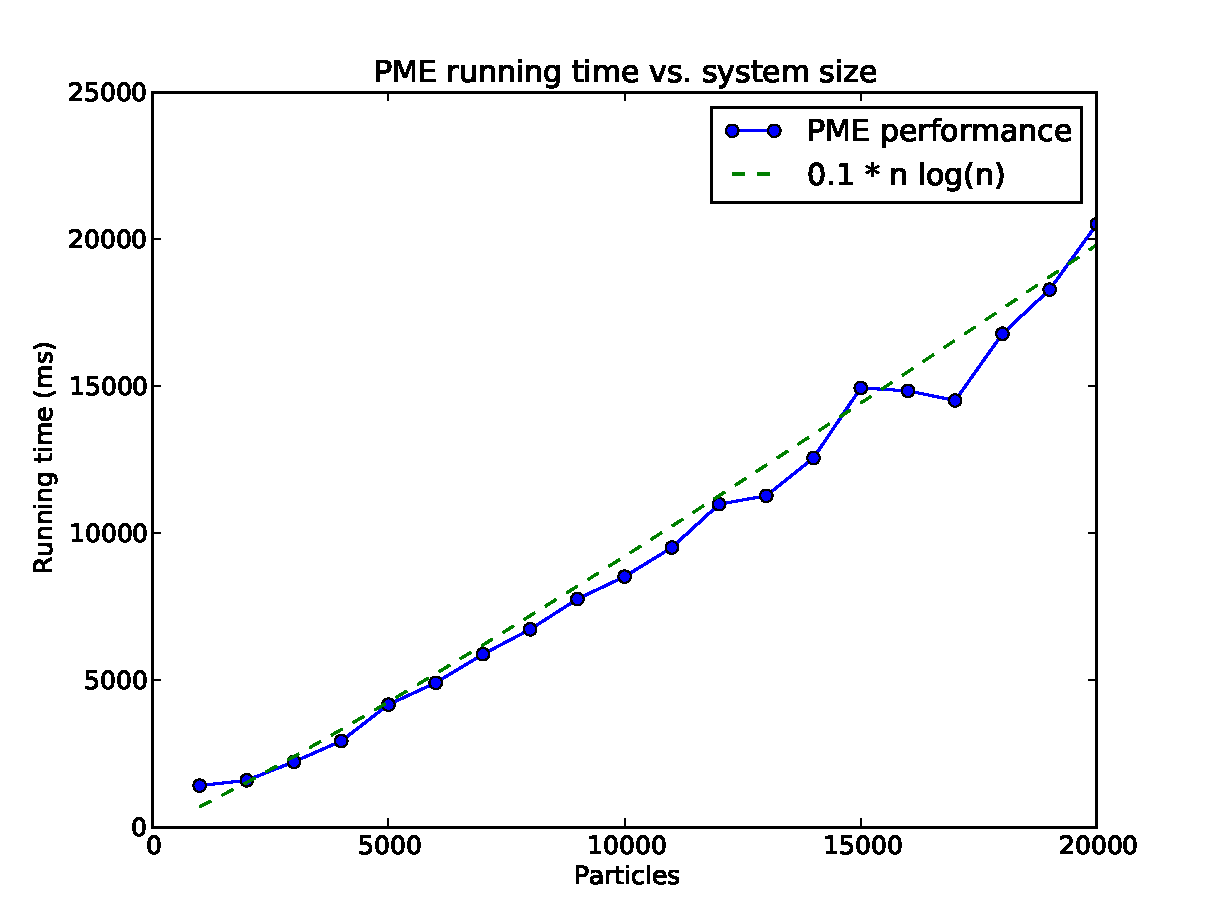
\includegraphics[width=0.75\textwidth]{figures/graphs/pme_algo_complex.pdf} \ecen
\caption{The running time of the \pmem{} with increasing system size}
\label{fig:pme_alg_complex}
\end{figure}
Figure \ref{fig:pme_alg_complex} shows the running time of the \pmem{}, with the hash table functions implemented. We can see that the rate at which the running time increases is proportional to $n\text{log}(n)$. It would be easy to fit a linear function to this data also, as in this range, $\text{log}(n)$ is a slowly growing factor compared to $n$.
\subsubsection{Method analysis}
We also present an analysis of the time taken by various functions in the \pmem{} using VisualVM\footnote{VisualVM, \url{http://visualvm.java.net/}}. (Table \ref{tab:pme_time_breakdown})
\begin{table}[h]
    \begin{tabular}{|l|l|l|}
        Method                       & Proportion of running time & Method description \\ \hline
        \texttt{pme.initQMatrix()}         & 53.2\%                      & Assigns charges to the grid using BSplines        \\ 
        \texttt{math.Complex.ln()}         & 43.6\%                      & Calculates $\text{log}(c)$             \\ 
        \texttt{math.initProximityList()}            & 3.2\%                      &  Compiles in range particle lists\\
    \end{tabular}
    \caption{The proportion of the running time spent in each method for the \fma while benchmarking.}
        \label{tab:pme_time_breakdown}
\end{table}
\subsection{Accuracy analysis}
The accuracy of the \pmem{} was far lower than expected in practice. Total energies calculated for systems had errors ranging from $1\%$ to $10\%$, depending on the system. Studying these systems led to the conclusion that the implementation of the reciprocal space calculation contains an error. It is likely that this error occurs in the generalisation from 3-Dimensions to 2-Dimensions, or in the exclusion of the self energy term \cite{essmann:8577}, which were compromises that had to be made to enable a truly direct comparison between the \pmem{} and the \fma{}. Figure \ref{fig:pme_acc} shows a visual representation of this discrepancy.
%%%%%%%%FIGURE%%%%%%%%%%%%%
\begin{figure}
\bcen 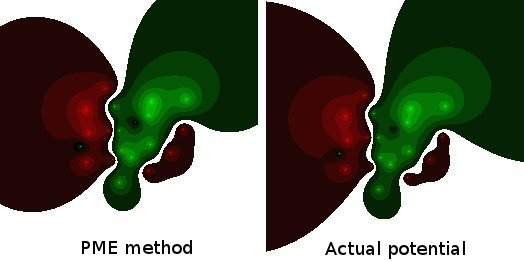
\includegraphics[width=0.75\textwidth]{figures/PMEscreenshot.jpg} \ecen
\caption{A visual comparison of the error of the \pmem{}. The different contours represent levels of potential.}
\label{fig:fig:pme_acc}
\end{figure}
%_________________ FMA SECTION __________________
\section{The Fast multipole algorithm}
\subsection{Background}
The \fma{} is similar to the \pmem{} in that both use a grid structure, and bounded approximations, to speed up computation. However, they are different in the ways they use the mesh, and the way approximations are made.
\subsubsection{Complex plane}
It should be noted that for this algorithm, it is simplest to implement in two dimensions. It is possible to to implement in three dimensions, with Spherical Harmonics \cite{Ihler04}, however this is not discussed in this paper. Instead, we work in two dimensions, on the complex plane. We give a point $(x,y)$ on the Real plane the value $z = x + yi$ on the Complex plane. This way, we can represent each point as a single number, and use complex versions of functions while calculating the multipole expansions.

\subsubsection{Multipole expansions}
A multipole expansion is a function which is a sum of a series of terms, which converges to some other function (in this case, the potential energy function). This convergence is fast, which makes it a good approximation to use in the \fma{}. These multipole expansions are centered on one point, and are valid for points within a certain distance of this center, but may be shifted and combined to gain more general multipole expansions. \cite{greengard:315}

\subsubsection{The mesh}
The mesh is similar to the one used in the \pmem{}. We say that the mesh has $n$ levels, and at each level we split each cell into quarters, starting with level $0$, which is the simulation cell. Each cell is split in four when moving down a level. We call the four sub cells of a cell $c$ the \emph{children} of $c$. Conversely, we call the cell that $c$ is a sub cell of the \emph{parent} of $c$.
%%%%%%%%FIGURE%%%%%%%%%%%%%
\begin{figure}[H]
\bcen 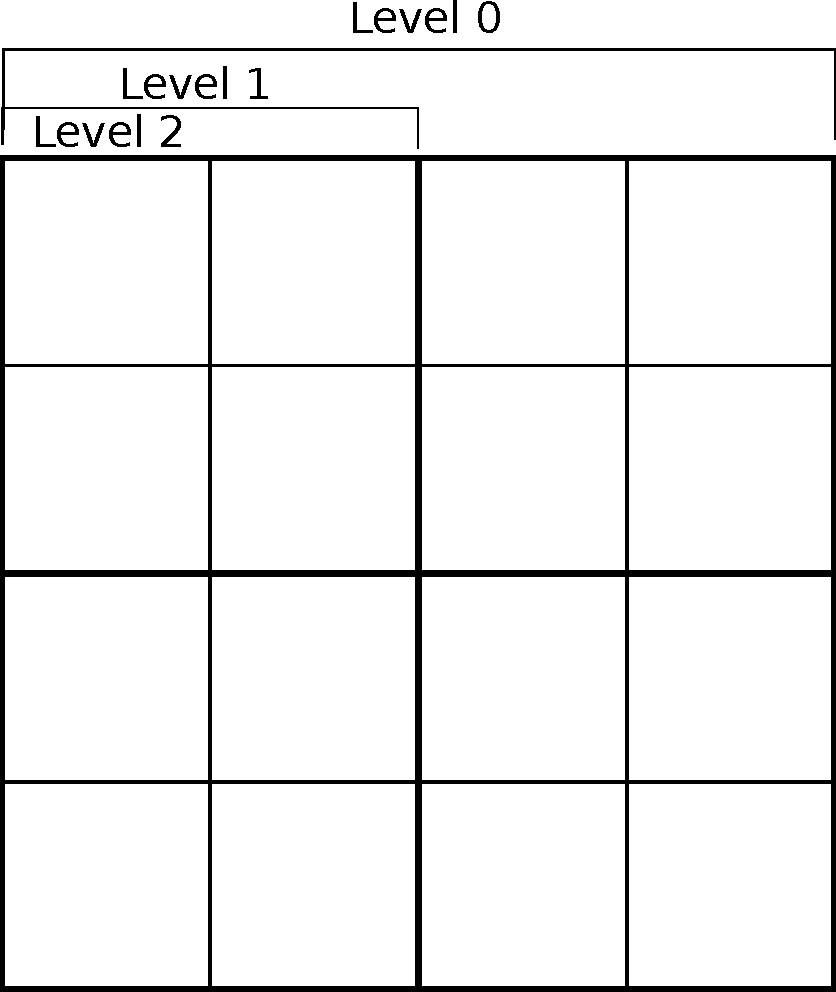
\includegraphics[width=0.35\textwidth]{figures/fma_mesh.pdf} \ecen
\caption{A simulation cell, with meshes up to level 2 displayed, giving $2^n = 2^2 = 4$ boxes per side}
\end{figure}

\subsubsection{Well separated cells}
\label{sec:well_sep}
For a cell $c$, we call a cell $d$ \emph{Well separated} from $c$ if\\
1) $\text{Parent}(d)$ is adjacent to $\text{Parent}(c)$ (adjacent horizontally, vertically or diagonally)\\
2) $d$ is not adjacet to $c$\\
\newline
These \emph{well separated} cells are the ones which we will use the expansions to calculate potential for. For cells that are not well separated, we will calculate interactions directly. Figure \ref{fig:pme_wellsep} gives an example of well separated cells.
%%%%%%%%FIGURE%%%%%%%%%%%%%
\begin{figure}[h]
\bcen 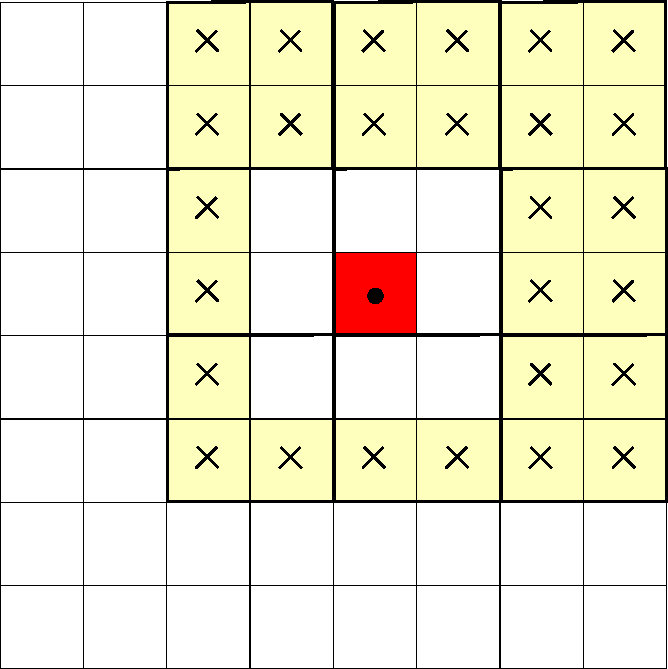
\includegraphics[width=0.35\textwidth]{figures/wellsep.pdf} \ecen
\caption{A cell, marked with a circle, and the squares that are well separated from it, marked with crosses.}
\label{fig:pme_wellsep}
\end{figure}

\subsection{Mathematical description}
\label{sec:fma_math}
\subsubsection{Potential and the multipole expansion approximation}
We describe the potential at a point $x_0 \in \mathbb{C}$ from the charge $q$ at $x \in \mathbb{C}$ by
\begin{equation}
\phi_{x_0}(x) = -q\text{log}{|x - x_0|}
\label{eq:potential}
\end{equation}
This function describes the logarithmic potential in 2-Dimensions. \cite{greengard:315} \cite{samaj}.\\

A multipole expansion for this function is derived in \cite{greengard:315}. Suppose that $m$ charges of strength $\{q_i,i=1,...,m\}$ are located at points $\{z_i, i=1,...,m\}$, with $|z_i| < r$. Then for any $z \in \mathbb{C}$ with $|z| > r$, the potential $\phi(z)$ is given by
\begin{equation}
\phi(z) = Q \text{log}(z) + \sum_{k=1} ^{\infty} \frac{a_k}{z^k}
\label{eq:multipole_expansion}
\end{equation}
Where
\begin{equation}
Q = \sum_{i=1} ^m q_i 
\hspace{0.5cm} \text{and} \hspace{0.5cm}
a_k = \sum_{i=1} ^m \frac{-q_i z^k _i}{k}
\end{equation}
While this is exact for an infinite sum of terms, we can truncate the series at term $p$, and if $p$ is large enough, this approximation is close to the actual potential $\phi(z)$. A description of how close can be found in \cite{greengard:315}
\subsubsection{Shifting multipole expansions}
A multipole expansion's center may be shifted, which is necessary for the \fma{}. Suppose that
\begin{equation}
\phi(z) = a_0 \text{log}(z-z_0) + \sum_{k=1} ^{\infty} \frac{a_k}{(z-z_0)^k}
\label{eq:pre_shift_multipole}
\end{equation}
Describes a multipole expansion which is centered on $z_0$. We can then shift this multipole expansion to be centered at the origin,
\begin{equation}
\phi(z) = a_0 \text{log}(z) + \sum_{l=1} ^{\infty} \frac{b_l}{z^l}
\label{eq:shifted_multipole}
\end{equation}
Where
\begin{equation}
b_l = \left(\sum_{k=1} ^l a_k z_0^{l-k} \binom{l-1}{k-1} - \frac{a_0 z_0^l}{l} \right)
\label{eq:b_descr}
\end{equation}
Note that this procedure of shifting to the origin is equivalent to shifting from any point $a$ to point $b$, if we treat point $b$ as the origin, and $a-b$ as our previous multipole expansion center.
\subsubsection{Local expansions}
We can find a local expansion about the origin due to a set of charges within radius $R$ of $z_0$, with $|z_0| > (c+1)R, \hs c > 1$. This local expansion is based on the multipole expansion at the same point.
\begin{equation}
\phi(z) = \sum _{l=0} ^{\infty} b_l * z^l
\label{local_expansion}
\end{equation}
Where
\begin{equation}
b_0 = \sum_{k=1} ^{\infty} \frac{a^k}{z^k_0} (-1)^k + a_0 \log(-z_0)
\label{where_local_expansion}
\end{equation}


\subsection{The algorithm}
\label{sec:fma_alg}
The basic flow of the algorithm is given below\\
%%%%%PSEUDOCODE%%%%%%%%%
\begin{algorithm}
\SetLine
\KwData{level-count: the number of mesh levels we create, $P$: the set of particles, $r$: a point at which we wish to calculate the potential}
\For{i=0 to level-count}{Initialise mesh[i] by adding all particles $p \in P$ to the appropriate cells}
\For{Each cell $c$ in mesh[level-count]}{Form a multipole expansion at at $c$, using Equation \ref{eq:multipole_expansion}}
\For{i=(levelcount-1) down to 0}{
    \For{Each cell $c$ in mesh[i]}{
        Shift each multipole expansion for the child cells of $c$ (in mesh[i+1]) to $c$ (Eq. \ref{eq:shifted_multipole})\;
        Combine and save these multipole expansions by addition\;
     }
}
\For{Each cell $c$ in mesh[0]}{
        Form a local expansion at $c$ based on $c$'s multipole expansion\;
        Shift $c$'s local expansion to the children of $c$\;
 }
\For{i=1 to level-count}{
    \For{Each cell $c$ in mesh[i]}{
        Shift $c$'s local expansion to the children of $c$\;
    }
}
Set the cumulative potential to 0\;
\For{Each cell $c$ in mesh[level-count]}{
    \eIf{$c$ is Well Separated from $d$'s cell}{
        Calculate the potential at $r$ from $c$'s local expansion\;
        Add this potential to the cumulative potential\;
    }{
        Calculate the potential at $r$ from $c$'s particles directly\;
        Add this potential to the cumulative potential\;
    }
}
Return the cumulative potential\;
\end{algorithm}

\subsection{The implementation}
A more object oriented approach was taken in the implementation of the \fma{} than in the \pmem{}. The primary classes the mathematics are \texttt{LocalExpansion.java} and \texttt{MultipoleExpansion.java}, which contain methods for creating, shifting, evaluating and storing the expansions described in Section \ref{sec:fma_math}.\\

An object for a mesh is implemented in \texttt{Mesh.java}, which contains a 2D array of cells, defined in \texttt{Cell.java}. The \texttt{Mesh} class contains a function called \texttt{makeCoarserMesh()} which creates a coarser mesh, shifting and merging multipole expansion in the process. This coarser mesh is saved into an array of each mesh level, from the maximum depth, to zero.

\subsection{Running time analysis}
\subsubsection{Complexity analysis}
The \fma{} was run over the class of problems with sizes in the range [0,5000] with an increment of 250, and [0, 20000] with an increment of 1000. The results are shown in Figure \ref{fig:fma_complex}.
%%%%%%%%FIGURE%%%%%%%%%%%%%
\begin{figure}
\subfigure[Range 0 - 2000]{ \label{fig:fma_complex_a} 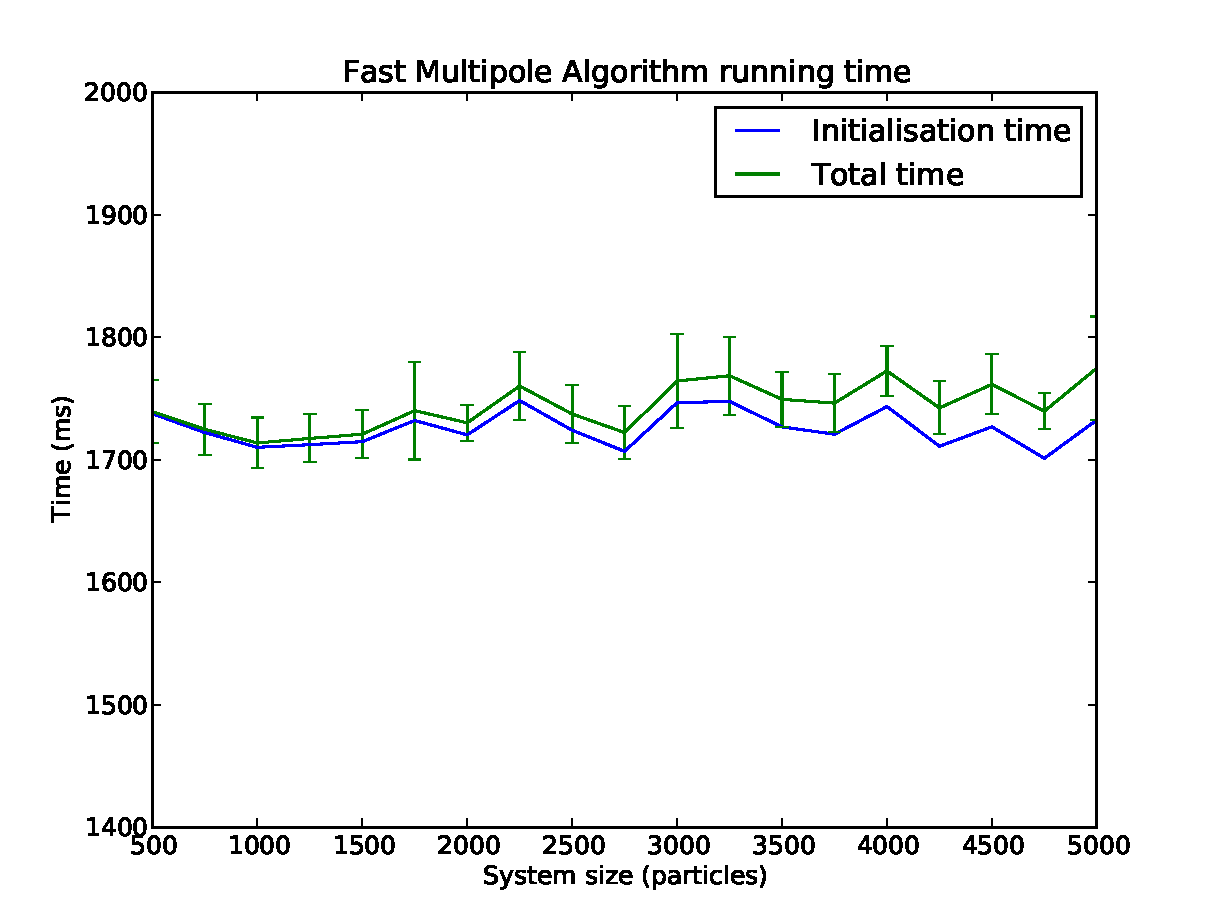
\includegraphics[width=0.49\textwidth]{figures/graphs/fma_0_5000.pdf}}
\subfigure[Range 0 - 20,000]{\label{fig:fma_complex_b} 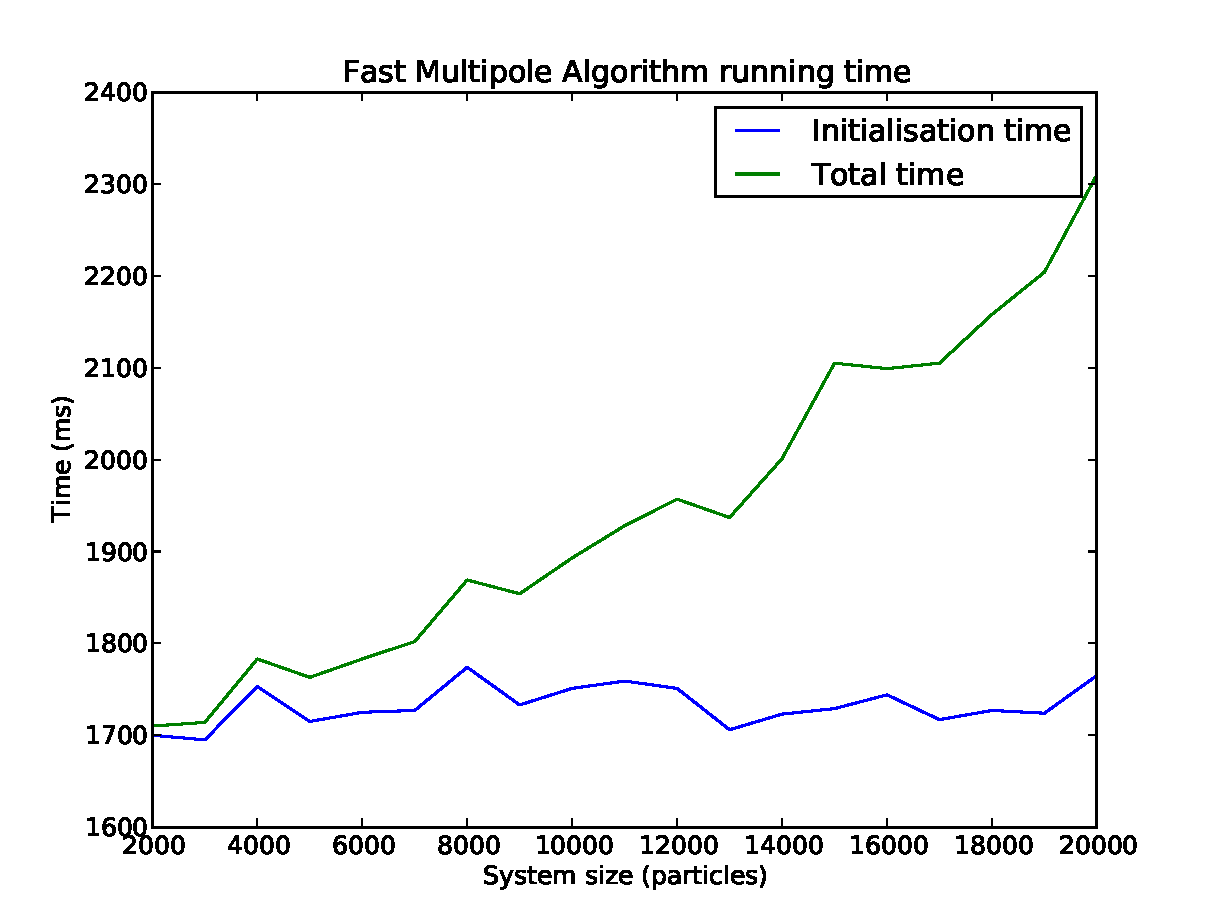
\includegraphics[width=0.49\textwidth]{figures/graphs/fma_2k_20k.pdf}}
\caption{The \fma's performance over the group of systems in the range 0 to 5,000 particles, and 0 to 20,000.}
\label{fig:fma_complex}
\end{figure}

The graphs here show the initialisation time and total time for the \fma{} on a set of problems. The initialisation time is the time required to compute the multipole and local expansions, and the total time is the initialisation time, with the time taken to evaluate these expansions included.

Figure \ref{fig:fma_complex_a} shows the same range as Figure \ref{fig:basic_algo_complex}, the basic algorithm's complexity. In it, we see that the initialisation time is taking most of the computation time. Each data point is an average of 20 trials, with the error bar indicating the standard deviation.

Figure \ref{fig:fma_complex_b} shows the \fma's run time for much larger problems, with up to 20,000 particles. We can see the initialisation time stay constant, while the total time grows linearly. So, we confirm that our implementation of the \fma is in the complexity class $O(n)$ \newline
\subsubsection{Method analysis}
Using \texttt{VisualVM} \footnote{VisualVM, \url{http://visualvm.java.net/}}, the table below of running times spent in each method was produced.

\begin{table}
    \begin{tabular}{|l|l|l|}
        Method                       & Proportion of running time & Method description \\ \hline
        \texttt{fma.LocalExpansion()}         & 31.6\%                      & Local expansion initialisation        \\ 
        \texttt{math.Complex.power()}         & 27.8\%                      & Calculates $c^x$             \\ 
        \texttt{math.Complex.ln()}            & 24.9\%                      & Calculates $\text{log}(c)$ \\
        \texttt{math.Binomial.binomial()}     & 9.6\%                       & Calculates binomial function \\ 
        \texttt{fma.MultipoleExpansion.add()} & 1\%                         & Adds multipole expansions
    \end{tabular}
    \label{tab:time_breakdown}
    \caption{The proportion of the running time spent in each method for the \fma while benchmarking.}
\end{table}

We can see that most of the running time is spent forming local expansions, and doing complex arithmetic. The run time is split over several different methods, which indicates there are no severe efficiency concerns. Most of the run time is spent performing complex arithmetic, which is what should be expected.

\subsection{Accuracy analysis}
The \fma{} has two main parameters that control accuracy - the number of mesh levels, and the number of terms in the multipole expansion. We call the number of mesh levels $N$ and the number of terms in the multipole expansion $p$. For reasonable accuracy, we should expect $N \approx \text{log}_4(n)$, where $n$ is the number of particles, and $p \approx \text{log}_2(\epsilon)$, where $\epsilon$ is the desired precision. \cite{greengard:315}
\subsubsection{Maximum mesh level}
We plot the accuracy of the method as a function of these two parameters. In figures \ref{fig:fma_mesh_acc} and \ref{fig:fma_fixed_mesh_acc}, we demonstrate the effect the mesh level has on the error. 

%%%%%%%%FIGURE%%%%%%%%%%%%%
\begin{figure}
\bcen 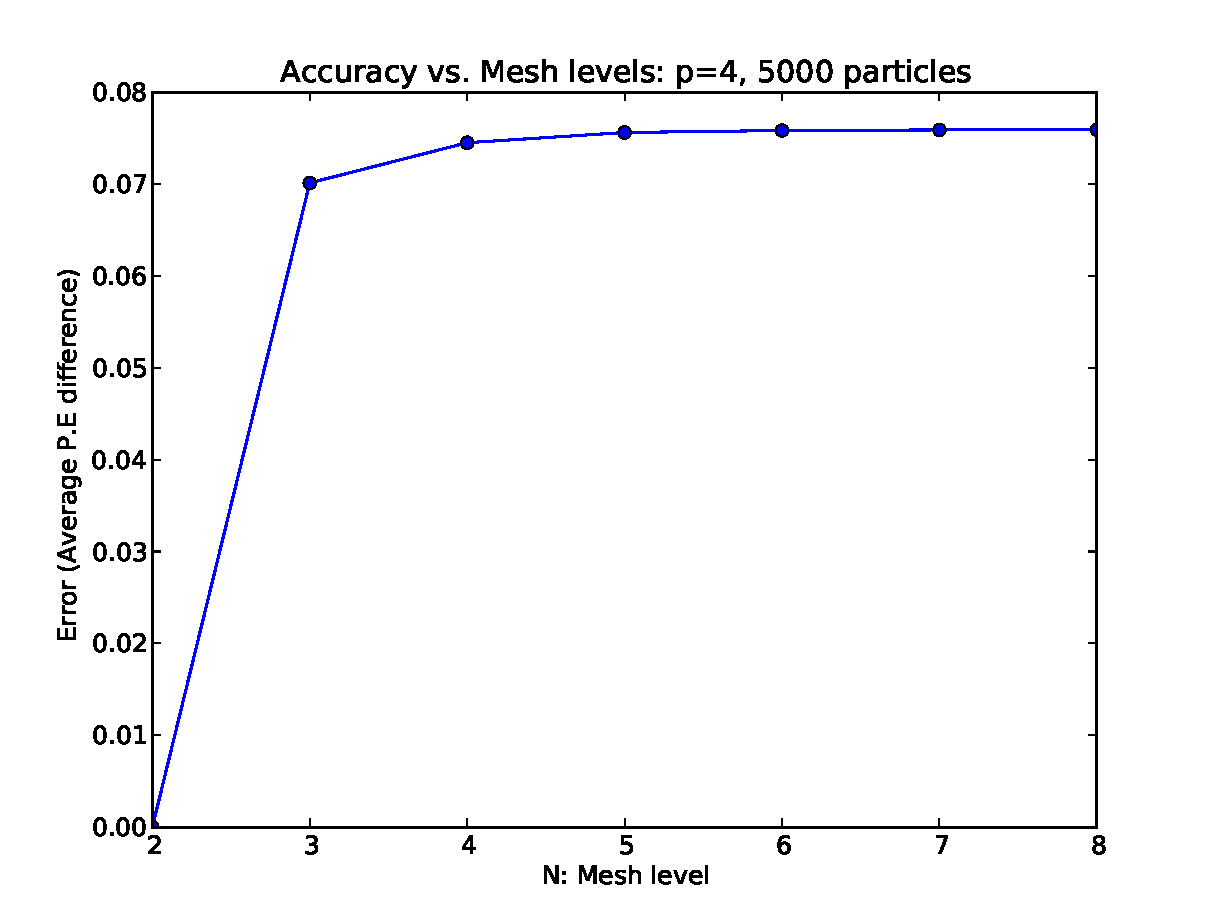
\includegraphics[width=0.75\textwidth]{figures/graphs/fma_mesh_acc.pdf} \ecen
\caption{The relationship between $N$, mesh levels, and the error, when comparied with the basic algorithm.}
\label{fig:fma_mesh_acc}
\end{figure}

Figure \ref{fig:fma_mesh_acc} shows the error \emph{increasing} with mesh level. This seems counter intuitive, however, according to The \fma{} from Section \ref{sec:fma_alg}, we calculate interactions directly for cells that are not well separated (See Section \ref{sec:well_sep}). With low mesh levels, such as $N=2$, this would include the entire simulation unit, which leads to the error of 0 we see at $N=2$. Increasing from here, we see the error level out to approximately 0.075. This graph shows that increasing maximum mesh level does not necessarily lead to improved accuracy.

%%%%%%%%FIGURE%%%%%%%%%%%%%
\begin{figure}
\bcen 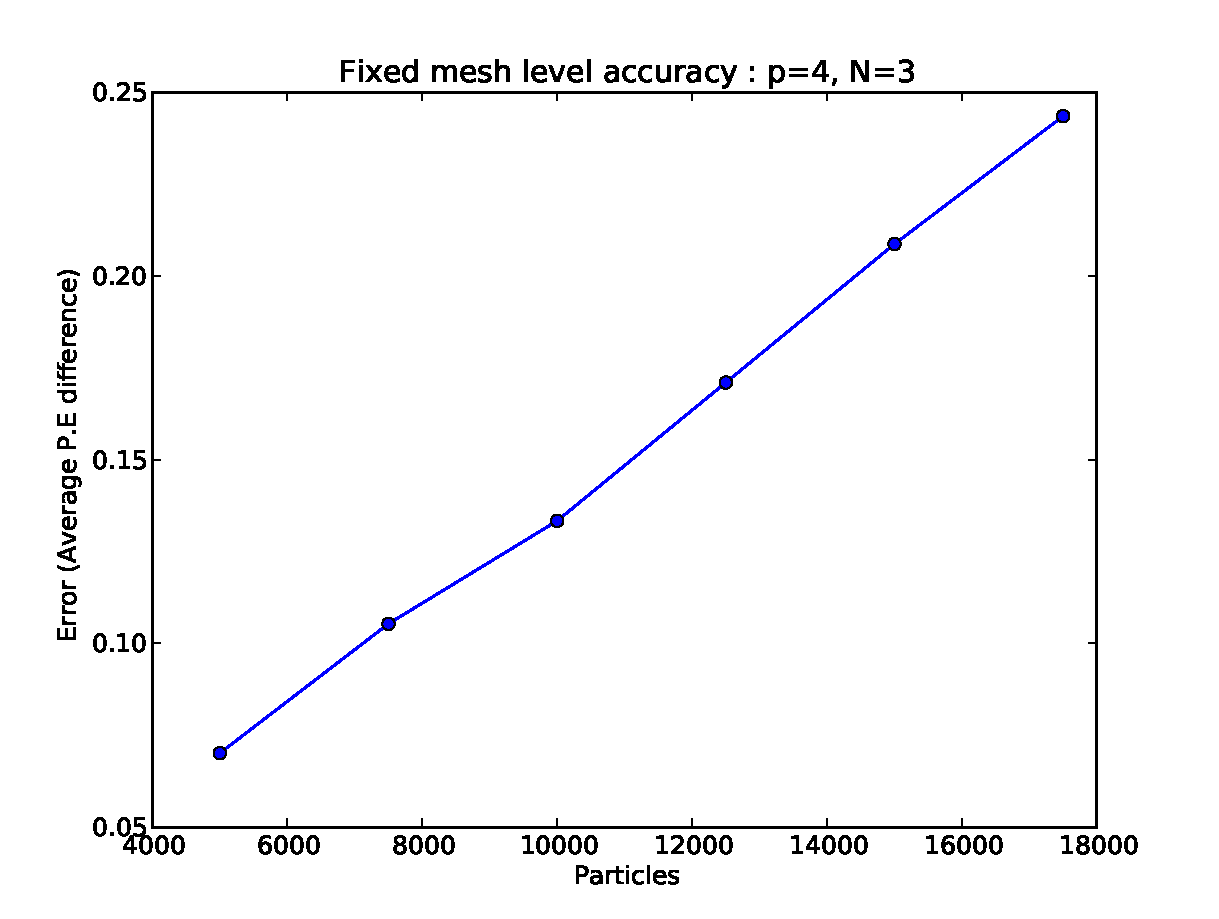
\includegraphics[width=0.75\textwidth]{figures/graphs/fma_fixed_mesh_acc.pdf} \ecen
\caption{The error for the \fma with a fixed mesh level $N=3$, with an increasing system size}
\label{fig:fma_fixed_mesh_acc}
\end{figure}

Figure \ref{fig:fma_fixed_mesh_acc} shows the effect of an increasing system size for a fixed $N$. We can see that the error grows linearly as we increase the number of particles if we keep $N$ and $p$ constant. From this we can confirm that a good rule is $N \approx \text{log}_4(n)$, with $n$ being the total number of particles in our system. This is recommended, as it keeps the number of particles per cell approximately constant. %TODO: a graph could show this.

\subsubsection{Number of terms}
Next we examine the effect the number of terms we truncate our multipole expansion at, $p$, has on the accuracy of our simulation.
%%%%%%%%FIGURE%%%%%%%%%%%%%
\begin{figure}
\bcen 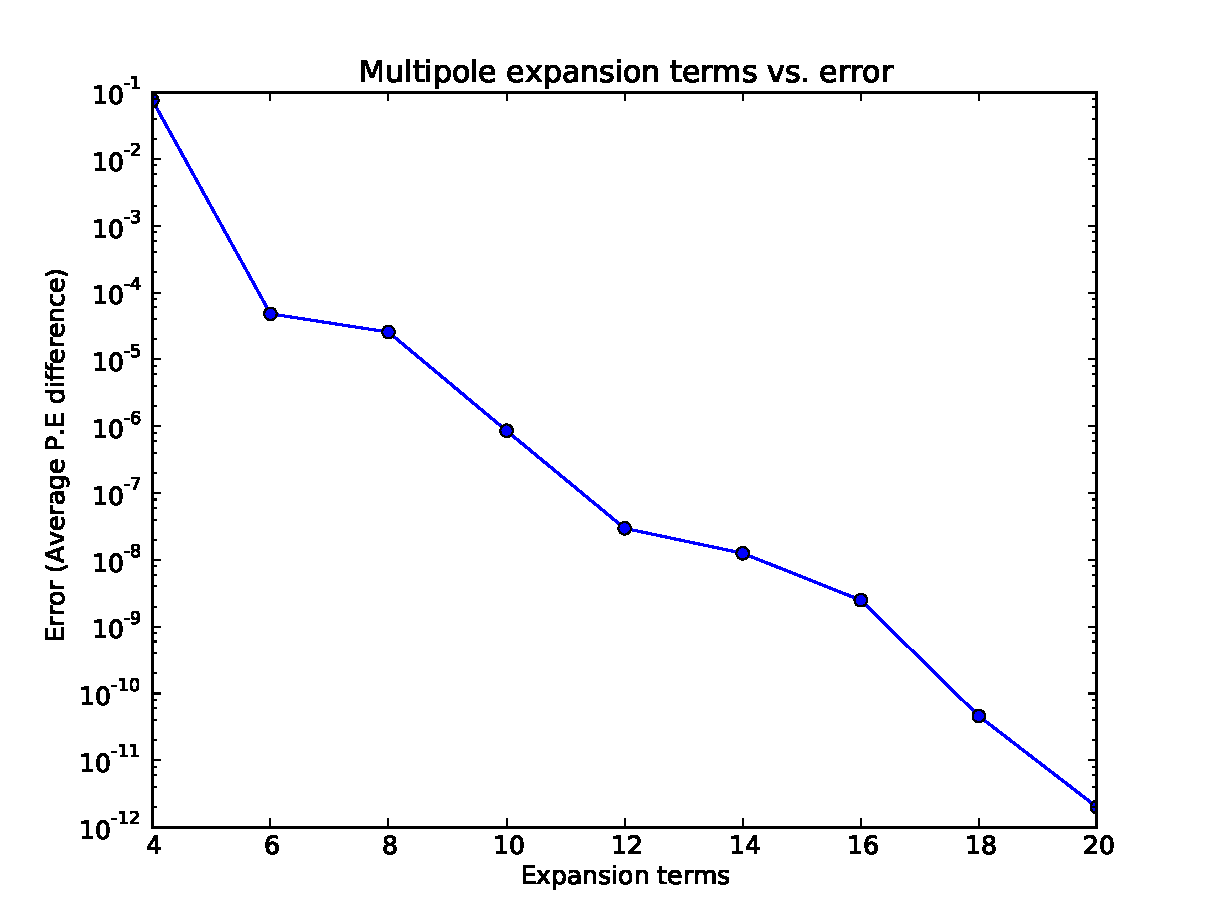
\includegraphics[width=0.75\textwidth]{figures/graphs/fma_terms_acc.pdf} \ecen
\caption{The error, on a logarithmic scale, vs. the number of terms in the multipole expansion, with a system size of 5000 particles}
\label{fig:fma_terms_acc}
\end{figure}

From Figure \ref{fig:fma_terms_acc} we see that the accuracy of the \fma{} increases exponentially as we increase the number of terms in our expansion. However, after $N \approx 20$, the improvement slows down. This is because we reach the machine precision in our accuracy at these levels.

%TODO: show the effect these parameters have on the running time?

\chapter{Comparison of the algorithms}
\label{chap:compare}
\section{Comparison of the running times}
\label{sec:run_comp}
The implementations were run on the same sets of data for different running times. The results of this experiment are shown in Figure \ref{fig:comp_graph}.
%%%%%%%%FIGURE%%%%%%%%%%%%%
\begin{figure}[H]
\bcen 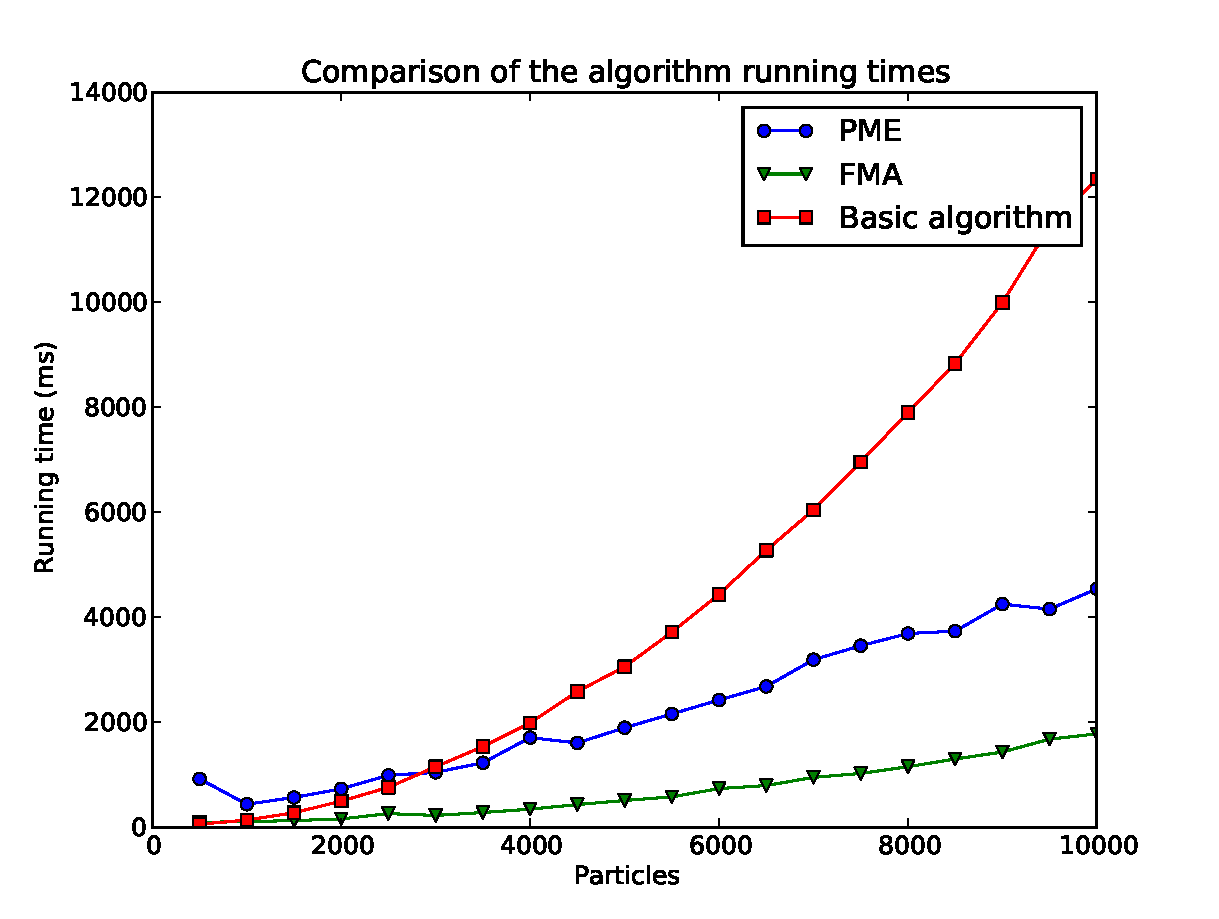
\includegraphics[width=0.75\textwidth]{figures/graphs/comp_graph.pdf} \ecen
\caption{A comparison of the running times for each algorithm, set to give accuracies on the order of $10^{-12}$, with increments of 500 particles, going up to 10,000 particles.}
\label{fig:comp_graph}
\end{figure}
The simulations were run on the systems ranging from 100 to 10,000 particles, and were set to give accuracies on the order of $10^{-12}$ (in the case of the \pmem, parameters were set to give a theoretical accuracy of $10^{-12}$ to ensure fairness in the experiment).

We can see from the graph that after a certain point, the implementations are ranked in the order of the Basic algorithm, the \pmem{}, and the \fma{}. Below $N=3000$ however, we see that the Basic algorithm is faster than the \pmem{}. After $N=3000$, the \pmem{} becomes faster.

To determine which algorithm is fastest for $N < 1000$, a higher resolution experiment was performed on these values. Figure \ref{fig:comp_graph_low} shows that the crossover point for the \fma{} and the \pmem{} occurs at approximately $N=750$. This is a small system size when it comes to practical simulations.

%%%%%%%%FIGURE%%%%%%%%%%%%%
\begin{figure}[H]
\bcen 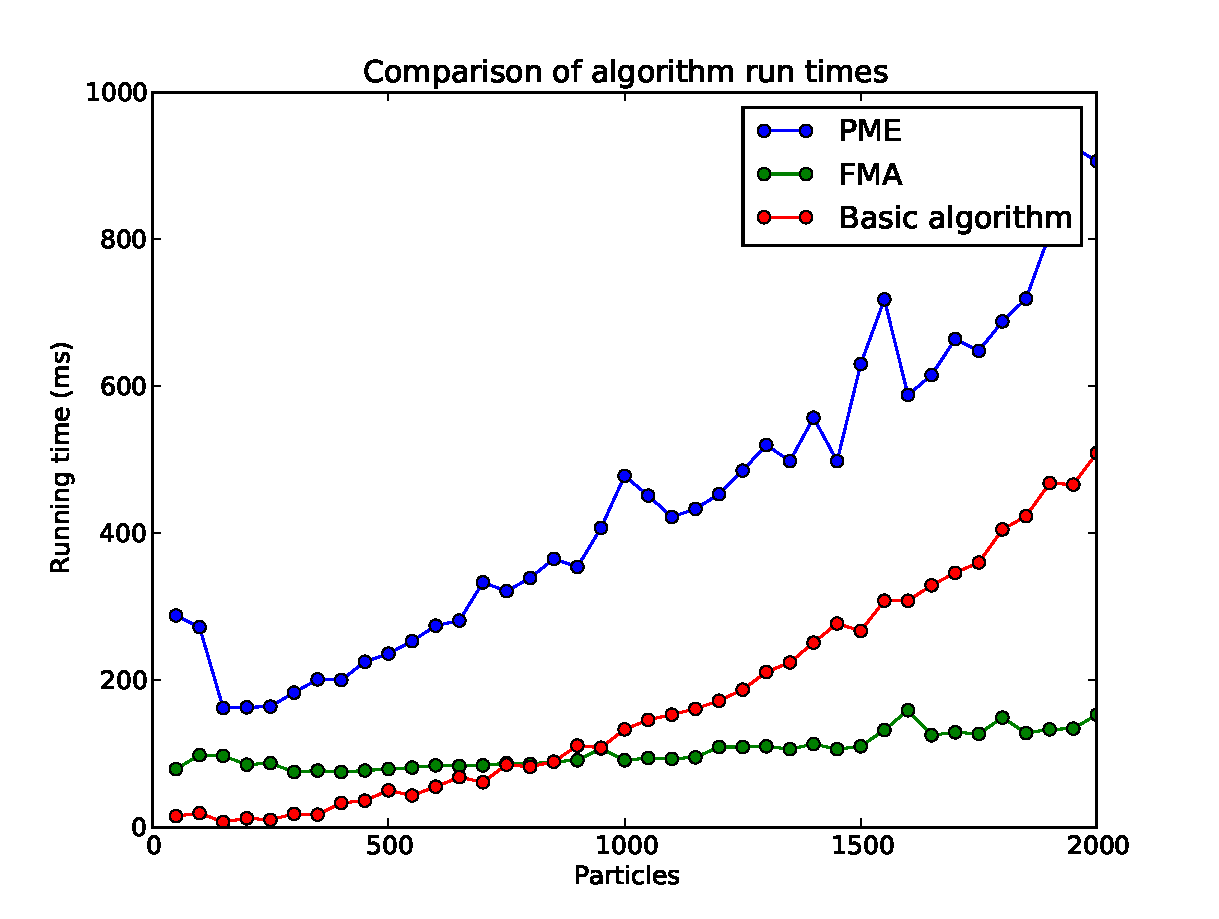
\includegraphics[width=0.75\textwidth]{figures/graphs/comp_graph_low.pdf} \ecen
\caption{A comparison of the running times for each algorithm, set to give accuracies on the order of $10^{-12}$, with increments of 50 particles, going up to 2000 particles.}
\label{fig:comp_graph_low}
\end{figure}
\section{Discussion}
\subsection{The \pmem{}}
\subsubsection{Advantages}
The \pmem{} has several features that differentiate it from the \fma{}. The first of these is Periodic Boundary Conditions (discussed in Section \ref{sec:pme_period_bound_cond}). Periodic Boundary Conditions allow simulation of large spaces realistically, with no reduction in performance. For practical applications, such as chemistry, boundary condition effects are dramatically reduced.

In addition to this, the \pmem{} as it is described in \cite{darden:10089} is described in three dimensions. The \fma{} requires the addition of Spherical Harmonics for the algorithm to be extended to 3-Dimensions \cite{spherical}, which increases the complexity of the algorithm, and the decreases the algorithm's efficiency.

Another advantage of the \pmem{} is it's suitability for parallel execution. Most of the calculations performed in the \pmem{} are independent of each other, and can be easily parallelised with a small amount of overhead (for example, the NAMD \cite{NAMD} molecular dynamics simulation software). Parallel methods for calculating the the Fourier Transformations are well explored \cite{lee05}.

\subsubsection{Disadvantages}
For some purposes, the Periodic Boundary Conditions introduce error rather than introduce it. This is the case for small systems, that should not tile infinitely in all dimensions. This was the case for the implementation presented in this paper, and padding was required to reduce the effects of the Periodic Boundary Conditions.

The mathematics of the \pmem{} is complex and intricate. This makes debugging, writing and maintaining software implementing the \pmem{} more difficult than for the \fma{}. 

While the \pmem{} has great potential to be optimised, it is easy to write suboptimal implementations \cite{toukmaji:73}. In place FFT, and careful use of floating point operations should be used to guarantee optimal performance \cite{lee05}. This was not implemented in this project, as readibility was preferred over marginal speed improvements.

\subsection{The \fma{}}
\subsubsection{Advantages}
The advantage of the \fma{} is it's $O(n)$ computational complexity, with a simple algorithm. We can see this in the graphs from Section \ref{sec:run_comp}, where the \fma{} performs best of the three algorithms examined.

\subsubsection{Disadvantages}
The \fma{} is not as simple to implement in 3-Dimensions, as it requires speherical harmonics \cite{spherical}. This brings extra computational time, and leads to a more complicated implementation.

The \fma{} is not as well suited to parallelisation as the \pmem{} is. The nature of the algorithm requires a tree structure, with each level dependent on the lower and higher expansions recursively.

\subsection{The Basic Algorithm}
\subsection{Advantages}
The Basic Algorithm is the fastest for systems with sizes in the range 0 to 750 (see Figure \ref{fig:comp_graph_low}). For small systems, this is the best choice of algorithm, as it has no initialisation time, and it's error is restricted only by the machine precision.

The Basic Algorithm is also well suited to parallelisation, and a parallel extension of the algorithm would be trivial, as particle-particle potential calculations are independent of each other.
\subsection{Disadvantages}
The obvious disadvantage to the Basic Algorithm is it's complexity of $O(n^2)$, which is inhibitive for most useful simulations. For molecular simulation, it is virtually impossible to use this approach.
\section{Conclusion}
For the system sizes tested, the Basic Algorithm was the fastest up to a system size with approximately 750 particles, and the \fma{} was consistently the fastest after this, by a factor of roughly 2 to 3. The \fma{} is recommended if algorithmic simplicity is sought, if the simulation environment is 2-Dimensional, or if a multi cpu architecture is not used.

However, the \pmem{} enjoys many advantages that cater it to high perfomance scientific computing, and particularly computational chemistry. While the \pmem{} is slower in this implementation, other implementations with a focus on optimisation could make the \pmem{} competitive with the \fma{}. 

%%%%%%_________APPENDICES____________
\appendix
\chapter{Implementation}
\label{ap:implement}
\section{Benchmark computer details}
\begin{table}[h]

    \begin{tabular}{l|l}
        CPU         & Intel(R) Core(TM) i7 CPU 950  @ 3.07GHz        \\ 
        L1 Cache                               & 256KB, 4-way set associative, write-through             \\ 
        L2 Cache                               & 1024KB, 8-way set associative, write-through \\
        L3 Cache                               & 8192KB, 16-way set associative, write-back \\ 
        Main memory                            & 6GB DDR3 1333Mhz\\ 
        Mflops/s                               & 64.424 Mflops/s
    \end{tabular}
    \caption{The relevant specifications for the computer used to benchmark the algorithms presented in the paper.}
\end{table}

%_______MATHS APPENDIX_______
\chapter{Algorithms and Mathematics}
\label{ap:math}
\section{The \pmem{}}

\subsection{Derivation of the reciprocal energy formula}
\label{ap:deriv_rec_energy}
The reciprocal space contribution to the electrostatic energy can be written as,\\
\begin{equation}
E_{\text{rec}} = \frac{1}{2*\pi*V} \sum_{m \not= 0} \frac{\text{exp}(- \pi^2 m^2 / \beta^2)}{m^2} B(m_1,m_2) S(m) S(-m)
  \label{eq:ap_primitive_rec_energy} \end{equation}
Where
\begin{itemize}
    \item $V$ is the volume (or in the two dimensional case, area) of the simulation cell,
    \item $\beta$ is the ewald coefficient,
    \item $S$ is the structure factor.
    \item $B$ is the matrix of B spline inverse fourier transform moduli, $B(m_1,m_2) = |b_1(m_1)|^2 * |b_2(m_2)|^2$. More detail on this can be found in \cite{essmann:8577}.
\end{itemize}
It is shown in \cite{essmann:8577} that $S(m) \approx F(Q(m))$, so we can rewrite this as a convolution\\
With this Q array we can calculate the long range contribution to the electrostatic potential in reciprocal space.\\

\begin{equation}
E_{\text{rec}} = \frac{1}{2} \sum_{m_1 = 0}^K \sum_{m_2 = 0}^K Q(m_1,m_2) * (\theta_{\text{rec}} \star Q)(m_1,m_2)
\label{eq:ap_energy_rec}
\end{equation}
With $\theta_{\text{rec}} = F(B * C)$, and so $(\theta_{\text{rec}} \star Q)(m_1,m_2) = F(B * C * F^{-1}(Q))$ \cite{essmann:8577} \cite{lee05}\\
Where $C$ is the matrix for the original exponential term from Equation \ref{eq:ap_primitive_rec_energy}, that is,
 \bcen
$\displaystyle
C(m_1,m_2) = \frac{1}{\pi V} \frac{\text{exp}(- \pi^2 m^2 / \beta^2)}{m^2} $ for $ m \not= 0, C(0,0) = 0$
\ecen 

\subsection{Evaluation of the B spline}
\label{sec:eval_bspline}
The recursive method for the calculation of the B spline is included here for completeness. See \cite{essmann:8577} \cite{lee05} for more details.

The B spline is defined by the following recurisve formula,
\bcen $\displaystyle M_2(x) = 1 - |x-1|$ for $0 \leq x \leq 2$, \hs $M_2(x) = 0$ for $u<0$ or $u>2$. \ecen
\[
M_n(x) = \frac{x}{n-1} M_{n-1}(x) + \frac{n-x}{n-1} M_{n-1}(x-1)
\]

The B spline's derivatives can also be calculated analytically. This is used in the force calculation.
\[
\frac{d}{dx} M_n(x) = M_{n-1}(x) - M_{n-1}(u-1)
\]


\subsection{Verlet list algorithm}
\label{sec:verlet}
The following algorithm utilises a list known as a \emph{Verlet list} to keep track of which particles are within a cutoff distance of each other, with only $O(n)$ complexity. It is used in the direct energy calculation of the \pmem{}\\
%%%%%PSEUDOCODE%%%%%%%%%
\begin{algorithm}
\SetLine
\For{i=0 to N}{
    $\text{cell}_x := \lceil u_{xi} \rceil$; (With $u_{xi}$ the scaled fractional x coordinate, as defined in Equation \ref{eq:q_array}))\\
    $\text{cell}_y := \lceil u_{yi} \rceil$; (With $u_{yi}$ the scaled fractional y coordinate))\\
    $\text{direct range} := \lceil r_{cut} / \text{mesh cell width} \rceil$\\
    \For{$\delta_x = -\text{direct range}$ to $+\text{direct range}$}{
        \For{$\delta_y = -\text{direct range}$ to $+\text{direct range}$}{
            \If{$\text{cell}_x + \delta_x$ and $\text{cell}_y + \delta_y$ are in the mesh}{
                Add i to the array closeParticles[$\text{cell}_x + \delta_x$][$\text{cell}_y + \delta_y$]
            }
        }
    }
}
\end{algorithm}
After this, the array closeParticles[x][y] contains all particles within $r_{\text{cut}}$ distance from a particle contained in mesh cell $x,y$.

\subsection{Ewald coefficient estimation algorithm}
\label{sec:alg_ewald_coeff}
The following algorithm uses a binary search to determine the best value of $\beta$ to use as the ewald coefficient by a binary search. Our goal is to satisfy the inequality in \ref{eq:ap_ewald_coeff} as closely as possible by modifying $\beta$.

\begin{equation}
\frac{\text{erfc}(\beta r_{\text{cut}})}{r_\text{cut}} \leq \epsilon_\text{tol}
\label{eq:ap_ewald_coeff}
\end{equation}

%%%%%PSEUDOCODE%%%%%%%%%
\begin{algorithm}
\KwData{$\epsilon_\text{tol}$: a tolerance value for our erfc term, $r_\text{cut}$: the chosen cutoff distance that is the border between direct and mesh based computation, $c$: some constant indicating how precise we wish the ewald coefficient to be.}
\SetLine
$\beta_\text{low} := 0$\\
$\beta_\text{high} := 1$\\
\While{$\displaystyle \frac{\text{erfc}(\beta_\text{high} r_\text{cut})}{r_\text{cut}} < \epsilon_\text{tol}$}{
$\beta_\text{high} := \beta_\text{high} * 2$
}
\vspace{0.25cm}
(At this point, $\beta_\text{low} \leq \beta \leq \beta_\text{high}$.)\\
\vspace{0.25cm}
\For{i:=0 to $c$}{
	$\beta := (\beta_\text{high} + \beta_\text{low}) / 2$\\
	\If{$\displaystyle \frac{\text{erfc}(\beta r_\text{cut})}{r_\text{cut}} > \epsilon_\text{tol}$}{
		$\beta_\text{high} := \beta$
	\Else{
		$\beta_\text{low} := \beta$
	}
	}
}
\Return{$\beta$}

\end{algorithm}

\bibliographystyle{plain}	
\bibliography{references}	

\end{document}
